\documentclass[]{article}

%packages
\usepackage{graphicx}
\usepackage{float}
\usepackage{sansmath}
\usepackage{amsmath, amssymb, amsfonts}

% Bibliographi
\usepackage{url}
\usepackage[numbers]{natbib}

\graphicspath{{../results/}, {../figures/}}

%opening
\title{MEMS: Lab1}
\author{Vilmer Dahlberg}
 
\begin{document}

\maketitle

\begin{abstract}

\end{abstract}

\section{Introduction}
Polycarbonates is a type of thermoplastic polymer which, due to its ease of use, high strength and toughness, can be found in many modern engineering applications \citet{wikipedia_polycarbonate}. To gain insight into the material properties of polycarbonate, we perform in this experiment a uniaxial tensile test. The specimen consists of a thin rectangular brick, with two circular notches in the center, shown in Figure \ref{fig:sample}.

Mention that we use a machine to load the specimen, and use displacement-controlled loading.

Mention something about how we record data using a lab-view program, and use a strain gauge to measure the force. 

Maybe talk about the type of material we are using?

\section{Method}
In this experiment we use a [what is this machine called] to load the specimen.

The specimen is a rectangular piece of polycarbonate with two semi-circle cut-outs [synonym to this], and is shown in figure [insert figure of specimen].

To begin we measure the specimens dimensions, which are given in the table [insert table of measurements].

The specimen is fastened into the machine by twisting the things, making sure to hold the arms such that no torsional loads are transferred to the specimen.

We then measure the height of the specimen. [but we only need this for the dic so not sure if i should mention it.]

The measuring software and tensile testing machine are then started at the same time. When the specimen fails the lab-view program and tensile test machine are then shut off.

\begin{figure}
	\centering
	\includegraphics[width=6cm]{Placeholder.png}
	\caption{Mosiac of experimental set-up}
	\label{fig:sample}
\end{figure}

\begin{figure}
	\centering
	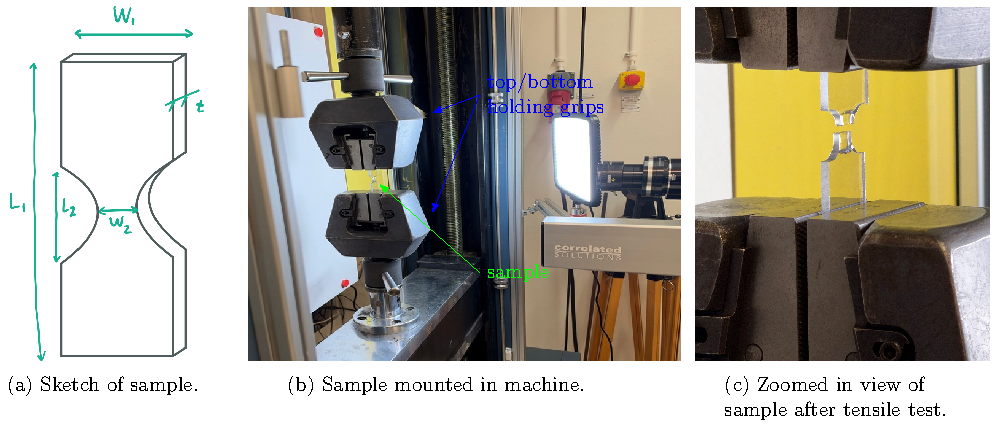
\includegraphics[width=10cm]{figure_mosiac.pdf}
	\caption{Mosiac of experimental set-up}
	\label{fig:method:setup}
\end{figure}

\section{Results}

These are the results
\begin{figure}[t]
	\centering
	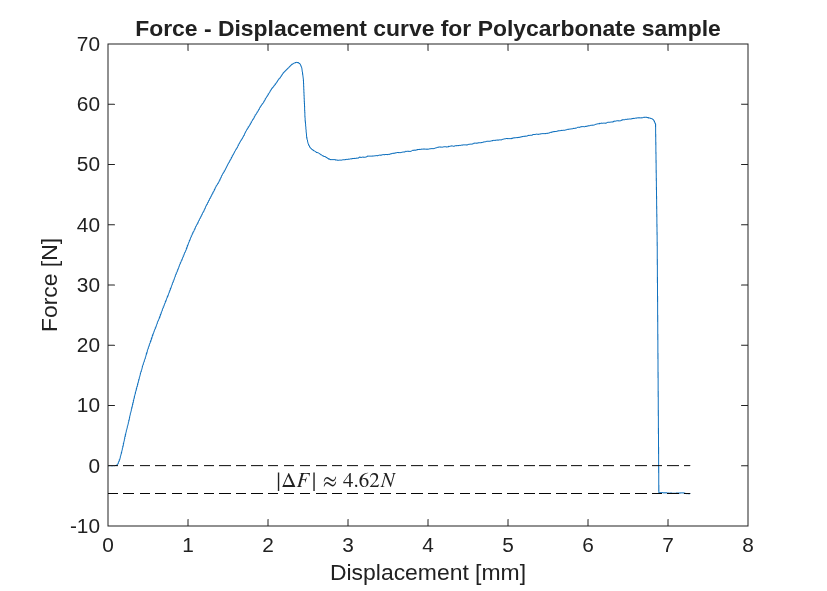
\includegraphics[width=10cm]{force_displacement.png}
	\caption{Plot of the force-displacement data gathered during the tensile test.}
	\label{fig:force_displacement}
\end{figure}


\section{Discussion}
Some points i would like to discuss.
\begin{itemize}
	\item[] You'd expect the curve to be linear initially, but it does not look like it. 
	\item[] Directly after the maximum load there is a decrease in force, this happens because we are using a displacement controlled loading. But maybe if we were to use a path following scheme we could trace the snap-back.
	\item[] After the drop there is a subsequent small increase in load, after failure finally occurs at circa 50N.
	\item[] What i personally find interesting is that we see no hysteresis, which is maybe what you would expect from polycarbonate.
	\item[] We also note (and maybe should begin with) the fact that we are looking at force-displacement data, and not a stress/strain relationship. Therefore it is hard to do any comparison between the results and any material model, which requires local data. This could be improved somewhat by doing a DIC, but the stress information is either way unknown.
\end{itemize}

\section{Conclusions}


\bibliographystyle{unsrtnat}
\bibliography{refs.bib}

\end{document}
